\documentclass[12pt,a4paper]{article}

%--------------------------------------------------
% Packages for layout, font, and graphics
%--------------------------------------------------
\usepackage[margin=1in]{geometry}
\usepackage{graphicx}
\usepackage{float}
\usepackage{setspace}
\usepackage{booktabs}
\usepackage{hyperref}
\hypersetup{
  colorlinks=true,
  linkcolor=black,
  citecolor=black,
  filecolor=black,
  urlcolor=black
}
\usepackage{caption}
\usepackage{titlesec}
\usepackage{tikz}
\usetikzlibrary{positioning,shapes.geometric,arrows.meta}
\usepackage{fontspec}
\usepackage{enumitem}
\usepackage{cite}
\usepackage{ragged2e}
\usepackage{array}
\usepackage[table]{xcolor}
\usepackage{tocloft}

%--------------------------------------------------
% Font and formatting setup
%--------------------------------------------------
\setmainfont{Trebuchet MS}
\setstretch{1.5}
\justifying

% Section formatting
\titleformat{\section}{\bfseries\fontsize{14}{16}\selectfont}{\thesection.}{0.5em}{}
\titleformat{\subsection}{\bfseries\fontsize{12}{14}\selectfont}{\thesubsection.}{0.5em}{}

% Table of contents formatting
\renewcommand{\cftsecfont}{\fontsize{14}{16}\selectfont}
\renewcommand{\cftsecpagefont}{\fontsize{14}{16}\selectfont}
\renewcommand{\cftsecleader}{\cftdotfill{\cftdotsep}}
\setlength{\cftsecindent}{0pt}
\setlength{\cftbeforesecskip}{6pt}

%--------------------------------------------------
% Begin Document
%--------------------------------------------------
\begin{document}

%--------------------------------------------------
% TITLE PAGE
%--------------------------------------------------
\begin{titlepage}
    \centering
    
\includegraphics[width=0.8\textwidth]{img/UCU.png}\\[1cm]
    
    {\Huge\bfseries Smart Fish Pond Management System}\\[1cm]
    {\LARGE\itshape  An IoT-Based Approach for Sustainable
 Aquaculture in Uganda}\\[1.5cm]
    
    {\Large\textbf{By:}}\\[1.2cm]
    {\Large\textbf{EZAMAMTI RONALD AUSTINE}}\\[0.5cm]
    {\large Registration No: S23B23-018}\\[0.5cm]
    {\large Access No: B24252}\\[1cm]
    
    {\Large\textbf{Course:} \\Embedded Systems and Microcontroller Programming-(BSCS-3)}\\[0.5cm]
    
\end{titlepage}

%--------------------------------------------------
% TABLE OF CONTENTS
%--------------------------------------------------
\renewcommand{\contentsname}{Table of Contents}
\tableofcontents
\clearpage

%--------------------------------------------------
% MAIN CONTENT
%--------------------------------------------------

\section{Project Title \& Problem Statement}
The \textbf{Smart Fish Pond Management System} addresses the persistent challenge of high fish mortality in Uganda's aquaculture, particularly for Nile tilapia (\textit{Oreochromis niloticus}) and African catfish (\textit{Clarias gariepinus}). Despite aquaculture growth in Uganda, smallholder farmers still record recurrent losses due to unstable water quality parameters—dissolved oxygen (DO), pH, temperature, turbidity, and ammonia—that affect fish metabolism and survival~\cite{tumwesigye2022effect, mramba2023pond}.

Uganda hosts more than 1,809 active cage fish units across Lake Victoria~\cite{clough2020innovative}, and pond systems continue to expand. However, water monitoring remains largely manual, relying on test kits or farmer observation. These methods are inconsistent and reactive, often detecting problems only after major losses have occurred. Between 2023 and 2024, the country's fish export volumes dropped by 27.8\%, and revenues fell by 21.9\%, primarily due to poor aquaculture productivity~\cite{byabasaija2025unlocking}. An affordable and automated monitoring solution is therefore essential to stabilize production and improve profitability.

\section{Relevance \& Stakeholders}
This project directly supports Uganda's \textbf{Vision 2040} and \textbf{National Development Plan IV (2025–2030)}, which prioritize ICT integration for agro-industrialization. Internationally, it contributes to:
\begin{itemize}
    \item \textbf{SDG 2:} Zero Hunger – through improved aquaculture yields.
    \item \textbf{SDG 6:} Clean Water and Sanitation – via sustainable pond management.
    \item \textbf{SDG 9:} Industry, Innovation, and Infrastructure – through local IoT innovation.
    \item \textbf{SDG 13:} Climate Action – using renewable solar power.
\end{itemize}

Primary stakeholders include smallholder farmers, the \textbf{Ministry of Agriculture, Animal Industry and Fisheries (MAAIF)}, producer organizations such as WAFICOS, and local aquaculture entrepreneurs. Secondary stakeholders are input suppliers, exporters, and research bodies promoting digital aquaculture technologies.

\section{Proposed Solution (Concept)}
The system integrates multiple sensors DO, pH, temperature, turbidity, and ammonia, connected to an ESP32 microcontroller with a GSM module for remote communication. It automatically regulates aeration and pumping whenever water parameters exceed safe limits. Farmers receive SMS alerts, allowing quick intervention~\cite{jomsri2024prototype}.

The system's architecture mirrors global IoT aquaculture frameworks~\cite{prapti2022internet, wang2021intelligent}, offering continuous data acquisition, low-cost scalability, and solar-powered autonomy. Designed for affordability and local assembly, it empowers smallholder farmers to manage ponds with precision while minimizing operational costs.

\section{Technical Feasibility}
The prototype uses an ESP32 MCU for data processing, DS18B20 temperature probes, DO/pH/turbidity sensors, and a SIM800L GSM module. Solar energy provides off-grid reliability. Firmware written in Arduino IDE will support threshold-based control, data logging, and communication features.

A field pilot will involve calibration using Wagtech or photometric reference kits, ensuring the sensors' accuracy and reliability under Ugandan pond conditions~\cite{aanyu2020potential}. The setup will also evaluate system performance against environmental fluctuations like rainfall and temperature shifts that affect pond oxygen levels.

\section{Societal \& Business Impact}
The proposed system enhances the efficiency and sustainability of smallholder aquaculture. It empowers farmers with real-time data to prevent fish kills, increases yields, and reduces dependency on imported technologies.  

Socially, it improves food security and rural incomes, while fostering youth innovation and employment in the assembly and maintenance of IoT devices. Economically, it contributes to restoring Uganda's declining aquaculture export share and aligns with regional trends in smart, sustainable fish farming~\cite{byabasaija2025unlocking, clough2020innovative}.

\section{Timeline}
The project will be implemented over five weeks:
\begin{itemize}
    \item \textbf{Week 1:} Literature review, design refinement, and component procurement.
    \item \textbf{Week 2:} Hardware interfacing, wiring, and testing of individual sensors.
    \item \textbf{Week 3:} Firmware programming and GSM integration.
    \item \textbf{Week 4:} Calibration, solar setup, and test deployment.
    \item \textbf{Week 5:} Field evaluation, performance analysis, and final report compilation.
\end{itemize}

\section{Draft Prototype Plan}
The prototype will consist of:
\begin{itemize}
    \item ESP32 microcontroller – data processing and control logic.
    \item Water quality sensors – DO, pH, turbidity, temperature, and ammonia.
    \item SIM800L GSM module – SMS alert and communication interface.
    \item Solar panel and battery unit – for continuous off-grid operation.
\end{itemize}
Testing will be performed on a demo tank before full deployment to an active pond. The system's success will be measured through reduced mortality and improved water quality stability.

%-------------------------------------------------- % 
% REFERENCES %
%-------------------------------------------------- %
\clearpage \newgeometry{margin=2cm} \renewcommand{\refname}{\centering\bfseries\fontsize{14}{16}\selectfont References} 
\addcontentsline{toc}{section}{References} 
\bibliographystyle{IEEEtran} 
\bibliography{SmartFish_References} 
\restoregeometry 
%-------------------------------------------------- % 
% APPENDIX %
%------------------------------------------------%
\clearpage 
\appendix \section*{\centering\bfseries\fontsize{14}{16}\selectfont Appendix} \addcontentsline{toc}{section}{Appendix}

\begin{figure}[H]
    \centering
    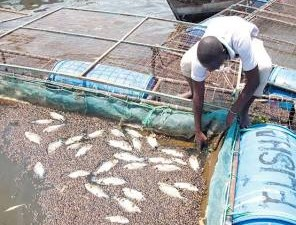
\includegraphics[width=0.5\textwidth]{img/low level.jpg}
    \caption{Low dissolved oxygen conditions leading to fish stress and mortality.}
    \label{fig:oxygen}
\end{figure}

\begin{figure}[H]
    \centering
    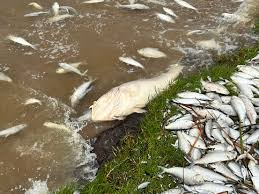
\includegraphics[width=0.5\textwidth]{img/dead fish.jpg}
    \caption{Mass fish mortality incident in Uganda caused by poor pond management.}
    \label{fig:deadfish}
\end{figure}

\begin{figure}[H]
    \centering
    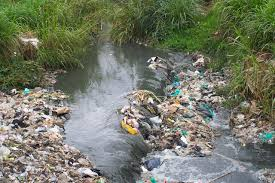
\includegraphics[width=0.5\textwidth]{img/waste.jpg}
    \caption{Waste buildup and turbidity increasing ammonia levels in pond water.}
    \label{fig:waste}
\end{figure}

\end{document}